\section{Imagen-Video}
\label{sec:imagen_video}

\begin{figure}
    \centering
    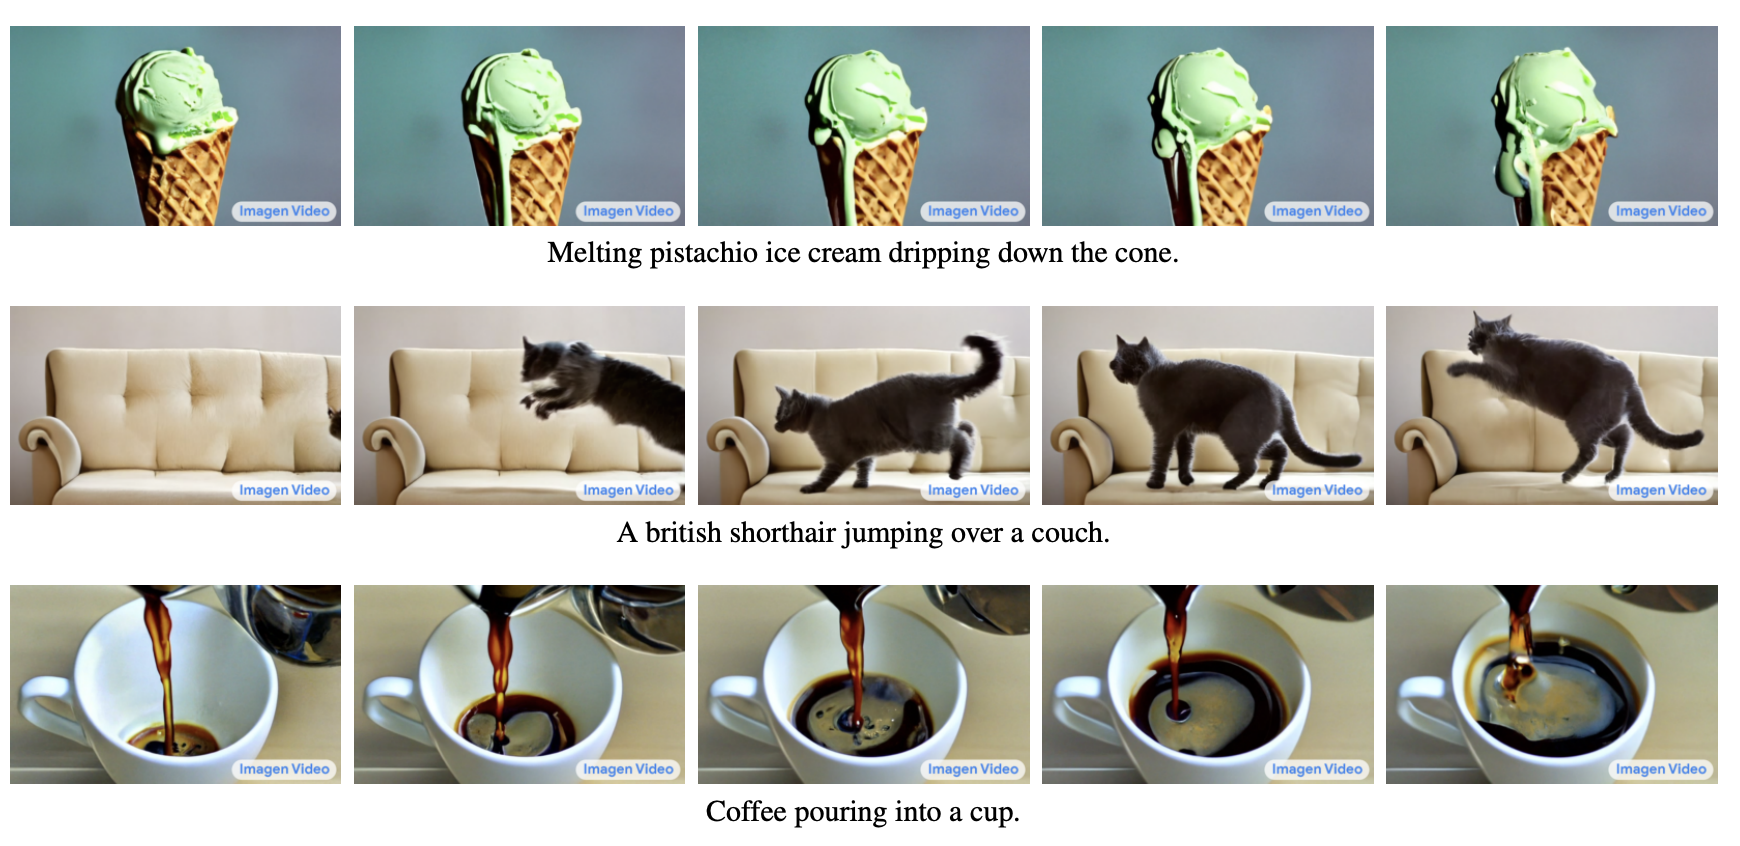
\includegraphics[width=1\textwidth]{images/video_synthesis/imagen_video.png}
    \caption{Imagen-Video video samples examples.}
\end{figure}

\begin{figure}
    \centering
    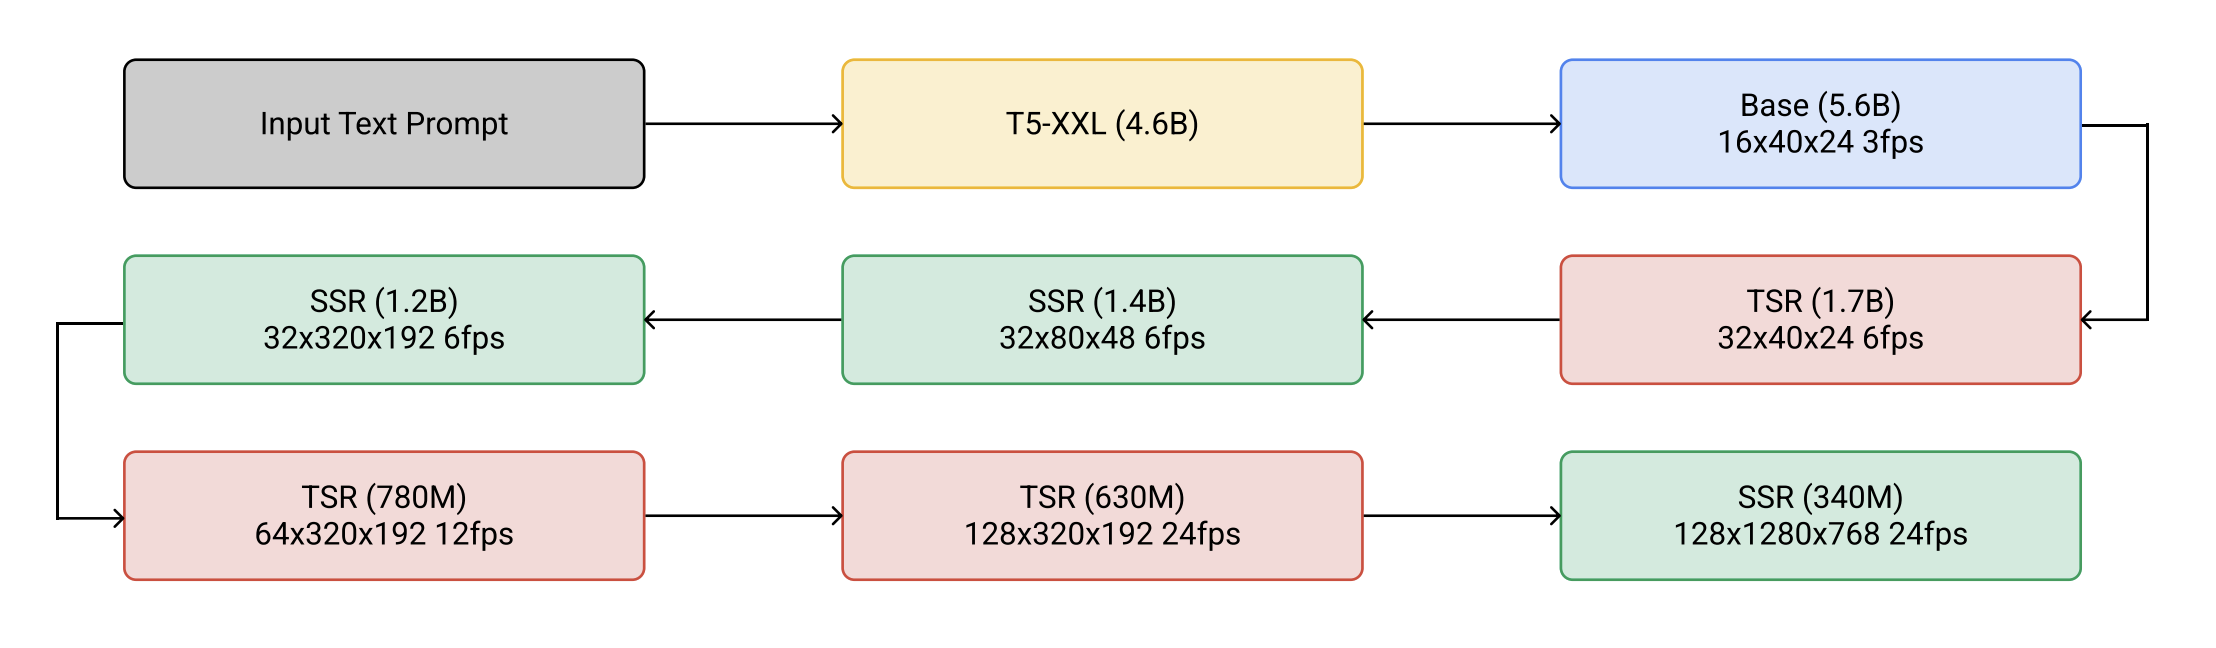
\includegraphics[width=1\textwidth]{images/imagen_video/pipeline.png}
    \caption{Imagen-Video cascading pipeline. The text embeddings are injected to all models in the pipeline (its not shown).}
    \label{fig:imagen_video_pipeline}
\end{figure}

Imagen-Video by Google \cite{imagen_video} is a text-to-video cascading diffusion model, based on previous work: Imagen (section \ref{sec:imagen}). It builds on the cascaded nature of Imagen. In total, Imagen-Video has 7 sub-models in a cascading pipeline (figure \ref{fig:imagen_video_pipeline}). Imagen-Video generates high definition $1280\times 768$ videos @ 24 fps, for 5.3 seconds. A big downside of Imagen-Video compared to Video-LDM is that Imagen-Video works in the pixel-space, whereas Video-LDM works in latent space. In addition, Imagen-Video is a much larger model and uses more resources than Video-LDM, however Google is able to achieve good results through massive training scaling.

Like Imagen, Imagen-Video uses the same large frozen text-encoder T5-XXL (section \ref{subsec:t5})in its pipeline.

The benefit of cascading pipeline is the ability to independently train each model, allowing the parallel training of all 7 models. Another benefit is the ability to use the super-resolution models, which are general purpose video super-resolution models, independently on downstream tasks.


\begin{figure}
    \centering
    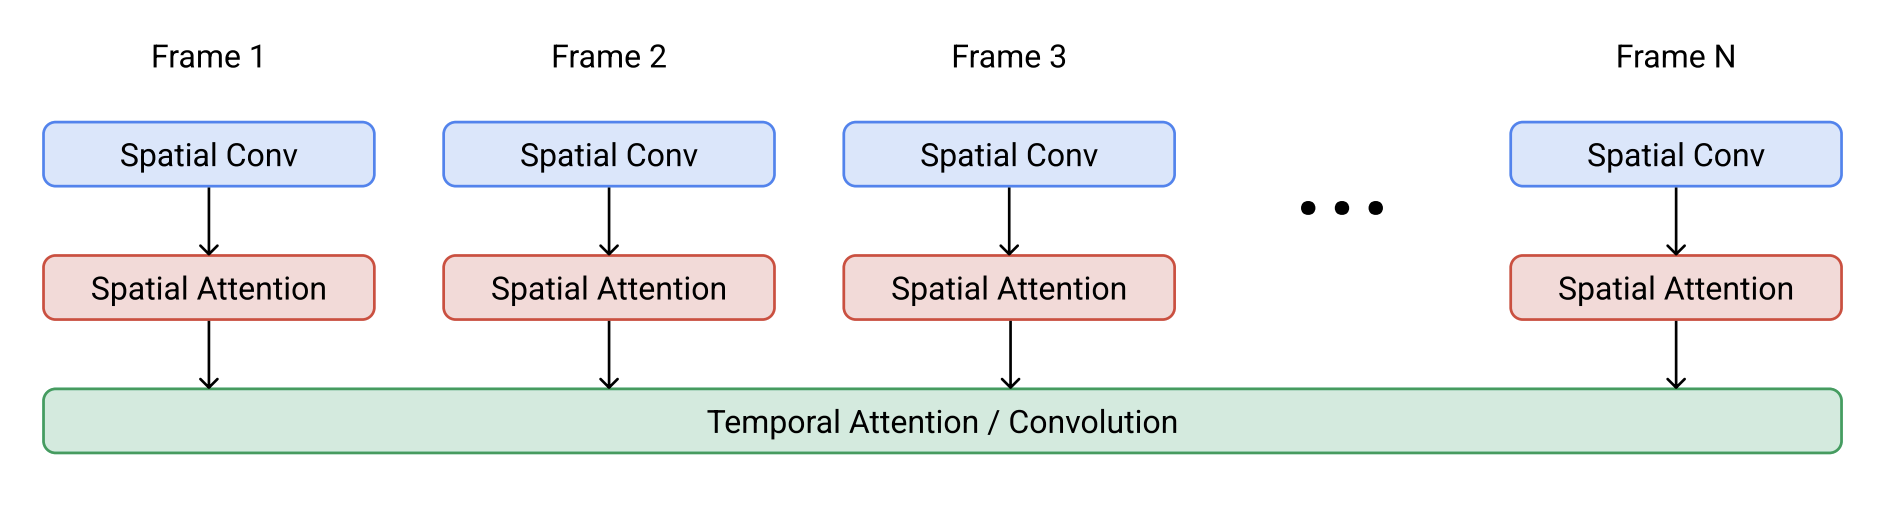
\includegraphics[width=1\textwidth]{images/imagen_video/video_u_net.png}
    \caption{Video U-Net block \cite{video_diffusion_models} used by Imagen-Video.}
    \label{fig:imagen_video_video_unet}
\end{figure}


Imagen Video also builds on the work of Video U-Net \cite{video_diffusion_models}, which generalizes the 2D diffusion model architecture to 3D in space-time by using temporal attention and 3D convolution layers to capture dependencies between video frames. See figure \ref{fig:imagen_video_video_unet}.









\subsection{Architecture}

Imagen Video has 1 frozen text encoder, 1 base video diffusion model, three SSR (spatial super-resolution) models, and three TSR (temporal super-resolution) models (totaling 7 video diffusion models).

Each of the denoising diffusion models $\hat{x_\theta}$ operate on multiple video frames simultaneously.

\textbf{Number of parameters:} Imagen Video consists of 11.6 billion parameters.

Imagen-Video pipeline is compromised of the following model types:

\begin{itemize}
    \item \textbf{T5-XXL:} As we discussed before, T5-XXL is a text-to-text transformer used to encode (text encoder) the text prompts to embeddings (tokens). 
    \item \textbf{Base:} The base model 
    \item \textbf{SSR:} The SSR model is a spatial super-resolution model that increases the resolution of the input image to higher spatial resolution.
    \item \textbf{TSR:} The TSR model increases the temporal resolution of the input video by filling in intermediate frames between the input frames.
\end{itemize}